\section*{PC farm status}

\begin{frame}{Code completely rewritten}{}
	\begin{itemize}
  		\item Thread-Thread and PC-Merger communications via ZMQ
  		\item Better logging
  		\item Some performance issues fixed
  		\item LKr double requests implemented (unicast and multicast)
  		 
	\end{itemize}
\end{frame}

\begin{frame}{Moved to github}{}
	\begin{columns}[t]
		\begin{column}{6cm}
		
				\begin{block}{git.cern.ch pretty awkward}
					Code available via https://github.com/NA62
				\end{block}
				
					\begin{block}{Code is open source}
						\begin{itemize}
				  			\item Free and easy download
				  			\item Registration suggested to contribute to the code 
						\end{itemize}
					\end{block}
	
		\end{column}
		\begin{column}{4cm}
			\vspace{-1cm}
			\begin{figure}[htp]
				  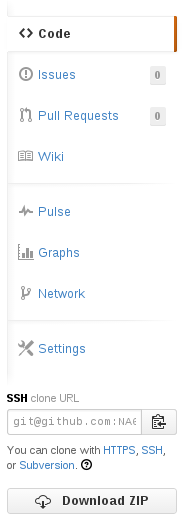
\includegraphics[width=2.5cm]{github.png}
			\end{figure}
		\end{column}
	\end{columns}

\end{frame}

\begin{frame}{Code structure}{}
	\begin{description}
  		\item[na62-farm-lib] All data formats defined here

  		\item[na62-trigger-algorithms] Playground for anybody implementing the
  		actual L1/L2 algorithms linking na62-farm-lib

  		\item[na62-farm] The actual software running on the farm linking na62-farm-lib
  		and na62-trigger-algorithms
  		
	  	\item[na62-trigger-test] Test project to execute trigger algorithms without
	  	the farm framework

  		\item[na62-farm-merger] The software running on the merger using
  		na62-farm-lib

  		\item[na62-farm-dim-interface] Interface for na62-farm and na62-farm-merger
  		to dim
  		 
	\end{description}
\end{frame}

\section*{Trigger algorithm development}

\begin{frame}{Documentation}{}
		\begin{block}{Wiki}
		Each project has it's own Wiki. E.g. trigger implementation:
		https://github.com/NA62/na62-trigger-algorithms/wiki/\ldots
		\begin{description}
  			\item[/GettingStarted] How to access the code and commit changes
  			
  			\item[/Structure] Coding guidelines and how to access the raw data within
  			the code
		\end{description}
	\end{block}
		
	\begin{block}{Bug tracker}
		Each project has its own bug tracker. E.g. trigger implementation:
		https://github.com/NA62/na62-trigger-algorithms/issues
	\end{block}
\end{frame}

\begin{frame}{Still new to git?}{}
	\begin{block}{Some nice pages for git beginners}
		\begin{description}
  			\item[A game to learn git] http://pcottle.github.io/learnGitBranching/
  			\item[Nice workflow]	http://danielkummer.github.io/git-flow-cheatsheet/
  			\item[Video] http://nvie.com/posts/a-git-flow-screencast/
		\end{description}
	\end{block}
\end{frame}

\begin{frame}{Next steps}{}
	\begin{block}{What I'm still waiting for}
		\begin{itemize}
  			\item Someone providing a MC to MEP converter
  			\item Someone developing L1/L2 trigger algorithms		
		\end{itemize}
	\end{block}
	
	Please contact me and I'll show you everything needed!
\end{frame}

\section*{Performance Tests}

\begin{frame}{Performance Tests}{}
	
	\begin{block}{Riccardo and Stefano did a few tests}
		So far only 400 kHz reached but only one sources sending (bad load balancing)
	\end{block}
	
	\begin{block}{Redesign still ongoing}
		The new code allows me to do better debugging and profiling
	\end{block}
	
	So far the merger seems to be the bottleneck (code still untouched since 2012!)
	\newline
	I will come to CERN next week to do more tests
\end{frame}